% Options for packages loaded elsewhere
% Options for packages loaded elsewhere
\PassOptionsToPackage{unicode}{hyperref}
\PassOptionsToPackage{hyphens}{url}
\PassOptionsToPackage{dvipsnames,svgnames,x11names}{xcolor}
%
\documentclass[
  10pt,
]{article}
\usepackage{xcolor}
\usepackage{amsmath,amssymb}
\setcounter{secnumdepth}{5}
\usepackage{iftex}
\ifPDFTeX
  \usepackage[T1]{fontenc}
  \usepackage[utf8]{inputenc}
  \usepackage{textcomp} % provide euro and other symbols
\else % if luatex or xetex
  \usepackage{unicode-math} % this also loads fontspec
  \defaultfontfeatures{Scale=MatchLowercase}
  \defaultfontfeatures[\rmfamily]{Ligatures=TeX,Scale=1}
\fi
\usepackage{lmodern}
\ifPDFTeX\else
  % xetex/luatex font selection
\fi
% Use upquote if available, for straight quotes in verbatim environments
\IfFileExists{upquote.sty}{\usepackage{upquote}}{}
\IfFileExists{microtype.sty}{% use microtype if available
  \usepackage[]{microtype}
  \UseMicrotypeSet[protrusion]{basicmath} % disable protrusion for tt fonts
}{}
\makeatletter
\@ifundefined{KOMAClassName}{% if non-KOMA class
  \IfFileExists{parskip.sty}{%
    \usepackage{parskip}
  }{% else
    \setlength{\parindent}{0pt}
    \setlength{\parskip}{6pt plus 2pt minus 1pt}}
}{% if KOMA class
  \KOMAoptions{parskip=half}}
\makeatother
% Make \paragraph and \subparagraph free-standing
\makeatletter
\ifx\paragraph\undefined\else
  \let\oldparagraph\paragraph
  \renewcommand{\paragraph}{
    \@ifstar
      \xxxParagraphStar
      \xxxParagraphNoStar
  }
  \newcommand{\xxxParagraphStar}[1]{\oldparagraph*{#1}\mbox{}}
  \newcommand{\xxxParagraphNoStar}[1]{\oldparagraph{#1}\mbox{}}
\fi
\ifx\subparagraph\undefined\else
  \let\oldsubparagraph\subparagraph
  \renewcommand{\subparagraph}{
    \@ifstar
      \xxxSubParagraphStar
      \xxxSubParagraphNoStar
  }
  \newcommand{\xxxSubParagraphStar}[1]{\oldsubparagraph*{#1}\mbox{}}
  \newcommand{\xxxSubParagraphNoStar}[1]{\oldsubparagraph{#1}\mbox{}}
\fi
\makeatother


\usepackage{longtable,booktabs,array}
\usepackage{calc} % for calculating minipage widths
% Correct order of tables after \paragraph or \subparagraph
\usepackage{etoolbox}
\makeatletter
\patchcmd\longtable{\par}{\if@noskipsec\mbox{}\fi\par}{}{}
\makeatother
% Allow footnotes in longtable head/foot
\IfFileExists{footnotehyper.sty}{\usepackage{footnotehyper}}{\usepackage{footnote}}
\makesavenoteenv{longtable}
\usepackage{graphicx}
\makeatletter
\newsavebox\pandoc@box
\newcommand*\pandocbounded[1]{% scales image to fit in text height/width
  \sbox\pandoc@box{#1}%
  \Gscale@div\@tempa{\textheight}{\dimexpr\ht\pandoc@box+\dp\pandoc@box\relax}%
  \Gscale@div\@tempb{\linewidth}{\wd\pandoc@box}%
  \ifdim\@tempb\p@<\@tempa\p@\let\@tempa\@tempb\fi% select the smaller of both
  \ifdim\@tempa\p@<\p@\scalebox{\@tempa}{\usebox\pandoc@box}%
  \else\usebox{\pandoc@box}%
  \fi%
}
% Set default figure placement to htbp
\def\fps@figure{htbp}
\makeatother





\setlength{\emergencystretch}{3em} % prevent overfull lines

\providecommand{\tightlist}{%
  \setlength{\itemsep}{0pt}\setlength{\parskip}{0pt}}



 
\usepackage[]{natbib}
\bibliographystyle{unsrt}


\usepackage[margin=1in]{geometry}
\usepackage{tikz}
\usepackage{adjustbox}
\usepackage{placeins}
\usepackage{appendix}
\usepackage{hyperref}
\usepackage{amsmath}
\usepackage{subfig}
\usepackage{booktabs}
\usepackage{longtable}
\usepackage{array}
\usepackage{multirow}
\usepackage{wrapfig}
\usepackage{float}
\usepackage{colortbl}
\usepackage{pdflscape}
\usepackage{tabu}
\usepackage{threeparttable}
\usepackage{threeparttablex}
\usepackage[normalem]{ulem}
\usepackage{makecell}
\usepackage{xcolor}
\makeatletter
\@ifpackageloaded{caption}{}{\usepackage{caption}}
\AtBeginDocument{%
\ifdefined\contentsname
  \renewcommand*\contentsname{Table of contents}
\else
  \newcommand\contentsname{Table of contents}
\fi
\ifdefined\listfigurename
  \renewcommand*\listfigurename{List of Figures}
\else
  \newcommand\listfigurename{List of Figures}
\fi
\ifdefined\listtablename
  \renewcommand*\listtablename{List of Tables}
\else
  \newcommand\listtablename{List of Tables}
\fi
\ifdefined\figurename
  \renewcommand*\figurename{Figure}
\else
  \newcommand\figurename{Figure}
\fi
\ifdefined\tablename
  \renewcommand*\tablename{Table}
\else
  \newcommand\tablename{Table}
\fi
}
\@ifpackageloaded{float}{}{\usepackage{float}}
\floatstyle{ruled}
\@ifundefined{c@chapter}{\newfloat{codelisting}{h}{lop}}{\newfloat{codelisting}{h}{lop}[chapter]}
\floatname{codelisting}{Listing}
\newcommand*\listoflistings{\listof{codelisting}{List of Listings}}
\makeatother
\makeatletter
\makeatother
\makeatletter
\@ifpackageloaded{caption}{}{\usepackage{caption}}
\@ifpackageloaded{subcaption}{}{\usepackage{subcaption}}
\makeatother
\usepackage{bookmark}
\IfFileExists{xurl.sty}{\usepackage{xurl}}{} % add URL line breaks if available
\urlstyle{same}
\hypersetup{
  pdftitle={Uneven Wage Growth and Public Goods},
  pdfauthor={Ebba Mark},
  colorlinks=true,
  linkcolor={blue},
  filecolor={Maroon},
  citecolor={Blue},
  urlcolor={Blue},
  pdfcreator={LaTeX via pandoc}}


\title{Uneven Wage Growth and Public Goods}
\usepackage{etoolbox}
\makeatletter
\providecommand{\subtitle}[1]{% add subtitle to \maketitle
  \apptocmd{\@title}{\par {\large #1 \par}}{}{}
}
\makeatother
\subtitle{The Case of US Public Education}
\author{Ebba Mark}
\date{}
\begin{document}
\maketitle

\begin{abstract}
 Wage growth is a key driver of local wealth accumulation, enabling greater household and community investment in public goods. Unfortunately, wage growth has diverged markedly from productivity growth in the United States in recent decades. As such, regions whose wages track productivity gains tend to benefit from broader economic growth, while lagging regions risk weaker savings capacity and declining support for public services. This work estimates the effect of local wage shocks on education spending using a shift-share instrumental variable design, exploiting variation in commuting zone industrial composition interacted with national industry growth shocks. We estimate that a 10\% increase in local wages generates a 2.3\% short-run increase in per-pupil education expenditure, with a long-run effect of approximately 4.6\%. This result is only driven by a handful of states, whereas others exhibit little wage responsiveness. These results expedite the need to enable education equalisation programmes to account for future potential wage disparities.
\end{abstract}

\renewcommand*\contentsname{Table of contents}
{
\hypersetup{linkcolor=}
\setcounter{tocdepth}{3}
\tableofcontents
}

\section{Introduction}\label{introduction}

\textbf{Since the 1970s, a persistent divergence between productivity
growth and wage growth has emerged in the United States
\citet{hoffmann2020}, \citet{stansbury},
\citet{economicpolicyinstitute}, \citet{elsby2013}.} While labour
productivity has continued to rise, the earnings of typical workers have
increased far more slowly, leading to a substantial decoupling between
the two trends. Economists cite various contributors to this phenomenon
from human capital \citet{autor2014}, \citet{katz1992},
\citet{acemoglu2012}, \citet{autor2011} to competition
\citet{stansbury}, \citet{deb2022}, \citet{yeh2022}, \citet{azar2022},
\citet{wilmers2018} to institutional and policy forces
\citet{egger2019}, \citet{lee1999}, \citet{mishel2021},
\citet{barkai2020}, \citet{autor2016}, \citet{card2001},
\citet{bivens2013}, \citet{stansbury2020} .\footnote{Summers \&
  Stansbury 2018 argue that productivity growth still exerts a positive
  influence on wages overall, but that institutional and structural
  changes have weakened the link for large segments of the workforce
  (\citet{summers2018} \citet{stansbury}). They point to declining union
  density, erosion of the minimum wage, globalization, and increased
  market concentration as key factors that have shifted bargaining power
  away from workers and reduced labour's share of national income
  \citet{autor2014}. Furthermore, additional evidence finds that this
  decoupling is far from a universal phenomenon. Rather, decoupling
  applies almost strictly to lower- and medium-wage earners, while
  already higher wages manage to keep up (relatively) with productivity
  growth rates.} Though its causes are hotly debated, the fact itself is
well-documented, especially for lower- and middle-income workers,
contributing to what is often termed the ``hollowing of the middle
class'' \citet{komlos2018}. \footnote{Though authors find that wage
  inequality growth has stagnated in the last decade this is not a
  result of a ``catch-up'' effect of lower- or middle-income earners
  with top income earners, but rather wage growth at the bottom of the
  wage distribution \citet{aeppli2022}. Additionally, further evidence
  indicates that metric choice can influence the ambiguity of earnings
  and wage inequality conclusions \citet{parolin2025}.}

\textbf{The direct consequences of this decoupling are clear.} Though
households and individuals often have stakes in firm productivity by
means other than wages, wages remain the most direct link between
aggregate productivity growth and local economic health. Therefore,
aggregate productivity growth is not sufficient to secure broad-based
improvements in living standards if the most direct link between
productivity and livelihoods is weak \citet{mishel2021}. Furthermore, in
a context in which the benefits of economic growth have already accrued
unevenly across communities in the United States by virtue of economic
history and industrial concentration, allowing this pattern to continue
could have adverse consequences for households and communities
\citet{bauluz}, \citet{rickard2020}, \citet{fee2025},
\citet{storper2009} \citet{fallah2011} \citet{benmelech}.

\textbf{A link that has been far less explored in this context is the
spillover effect of local wages to local wealth-building and its effect
on public goods.} Wage growth is an important contributor to local
wealth-building, allowing households and communities to invest more in
local public goods \citet{boustan2013}. Communities whose wages rise in
line with productivity growth will likely reap the benefits of economic
growth whereas those who do not, risk falling behind. This link is
particularly important in the US given the structure of local public
financing. Majority of local public services are funded via property
taxes. This funding structure entrenches a mechanism for generating
inequality of opportunity between diversely affluent regions of the
country \citet{manduca2025} \citet{weir2021} \citet{schechtl2024}
\citet{mettler2011} .\footnote{A burgeoning literature points to the
  role of racial segregation and its enduring legacy in perpetuating
  inequality in local economic health, wealth, and public service
  expenditure \citet{avenancio-león2022} \citet{trounstine2016}
  \citet{trounstine2021} .} Put plainly, given the structure of US
public services, wherein they are tied to asset values, inequality in
wealth-building can have significant effects for the quality of local
public services. Furthermore, a sometimes lacking, or at best
under-performing, federal equalisation systems perpetuates this
structural force \citet{beland2017} \citet{biasi2023} \citet{hoxby1998}
\citet{mccabe2019} \citet{baker2016} .

\textbf{Community well-being and public expenditure in the US is already
characterised by a high degree of spatial heterogeneity
\citet{manduca2025}, \citet{obrien2025}, \citet{feler2017} .} Evidence
of how income inequality perpetuates other forms of inequality
(opportunity, health, infrastructure quality, and broader well-being) is
steadily increasing \citet{chetty2016}, \citet{logan2012},
\citet{semuels2016}, \citet{Avancena2021}, \citet{flavin2009}.
\citet{boustanEffectRisingIncome2013} find that greater income
inequality leads to higher public expenditure across all public goods
indicating that a presence of higher-earners in a local area contributes
to higher levels of expenditure. Though this does not support an
unambiguous denunciation of inequality in itself, it provides additional
evidence for the fact that local incomes affect public expenditure
raising the potential for ``superstar'' and ``left behind'' regions to
emerge absent even income growth.

\textbf{One public service that has particularly important ties to
ensuring generational resilience to economic decline is education.}
Public schools around the US are responsible for educating over 80\% of
school-age children. In 2019, governments around the US (including the
federal government) spent a total of \$870 billion on public education,
roughly \$17,013 per pupil
\citet{nationalcenterforeducationstatistics2023}. However, the quality
of services delivered varies widely across the country
\citet{biolsi2022}. Take Connecticut for example. In 2016, according to
the Connecticut State Department of Education, the town of Greenwich
town, one of the highest-income towns in the country, spent \$22,000 per
pupil while Bridgeport, although only located 40Km away, spent \$14,000
\citet{semuels2016}.

\textbf{The quality of public education, especially at an early age, can
have long-lasting consequences for personal and economic well-being over
an individual's lifetime as well as generations following them
\citet{alfonso2020}, \citet{zheng2022}\citet{unicef} .} Although only a
small piece of the puzzle that determines quality public education,
expenditure levels ensure adequate funding for facilities, teachers,
administrators, and other services \citet{baker2017} \citet{baker2025}
\citet{jackson2016} . Furthermore, evidence suggests that progressive
spending delivers efficiency gains in school performance
\citet{rauscher2022} . Therefore, ensuring that local or regional
economic decline does not disrupt or worsen the quality of education
delivered is of paramount importance to ensure greater equality in the
long-run. Altogether, this evidence points to the value of identifying
the extent to which expenditure on public education is reliant on local
wage growth across the country.

\textbf{This study therefore determines whether elasticities of public
elementary education expenditure to local wage growth are non-zero.} If
productivity gains translate unevenly into wages across regions, then
the fiscal capacity of local governments may be shaped as much by
institutional and structural conditions as by the distribution of
aggregate economic growth. We investigate the following questions:

\emph{RQ1:} Do local wage gains affect public education expenditure in
levels?

\emph{RQ2:} If so, is this relationship constant across commuting zones?
What sources of heterogeneity mediate this relationship?

\emph{RQ3:} In light of recent reforms to intergovernmental education
funding aimed at reducing disparities in educational expenditure, do
intergovernmental transfers mitigate wealth-driven inequalities in
public education spending?

\subsection{Theoretical Motivation and Empirical
Approach}\label{theoretical-motivation-and-empirical-approach}

Any study of the linkage between two or more local socio-economic
outcomes presents considerable endogeneity challenges. In the context of
this study, wages and public education expenditure are undoubtedly
endogenous. Higher-income families may self-select into districts with
greater education spending, confounding causal inference. Lower-income
families likely struggle financially to make similar mobility decisions.
Local education contributes to the quality of local human capital
impacting wages and potentially preferences for education.

Therefore, we approach causal identification by instrumenting local
wages using a shift-share instrumental variable design. More precisely,
to interrogate the elasticity of public education expenditure to wages
across US commuting zones, we construct a shift-share instrument that
combines fixed local industry employment shares with national
industry-level changes real value added using data from the US Bureau of
Labor Statistics and Bureau of Economic Analysis. This instrument
generates plausibly exogenous local variation by exploiting how
different regions are differentially exposed to common national trends,
while abstracting from endogenous local dynamics. It is particularly
well suited in this setting, since the local tax base, and thus
education spending, likely depends on industries that are unevenly
distributed across regions but subject to similar industry-specific wage
shocks. Finally, we use this instrument to identify the effect of wage
shocks on local public education expenditure as reported by the US
Census Bureau's Annual Survey of State and Local Government Finances.

Given the substantial heterogeneity across U.S. states arising both from
structural sources (such as differences in tax systems, regulatory
environments, and legislative institutions) and from evolved
characteristics (including industrial composition, income levels,
inequality, and broader measures of economic diversity) the scope for
identifying a policy-relevant single national average treatment effect
is inherently limited. Therefore, we proceed in two steps. First, we
provide an initial benchmark using a pooled estimation to establish a
baseline relationship between wages and education expenditure that
generalizes reasonably across the national economy. Second, we
investigate the regional and industrial heterogeneity that these pooled
estimates mask via a state-by-state estimation, industry-by-industry
estimation, and grouping commuting zones by their historic wage and GDP
growth trajectories to improve comparability of treatment and control
groups in our instrumental variable design. In the latter heterogeneity
analysis, we construct commuting zone growth rates as idiosyncratic
variables absent state and national-level growth rates, understanding
that \emph{relative} growth rates are of particular importance in a
landscape where local economies determine the actual \emph{value} of
wage levels.

\subsection{Detailed results}\label{detailed-results}

\begin{enumerate}
\def\labelenumi{\arabic{enumi}.}
\tightlist
\item
  Public education expenditure is not agnostic to local economic
  conditions. We establish a strong positive causal link between public
  education expenditure and local wages, wherein a 10\% increase in
  local wages drives a 2.2\% increase in public elementary education
  expenditure, with a long-run increase of 4.6\%.
\item
  Estimating the instrumental variable model separately for each state
  reveals substantial heterogeneity in the relationship between wages
  and education expenditure. Only a third of the 40 states analysed in
  this study show persistent causal relationships between wages and
  education expenditure, indicating that these carry the weight of
  national-level identification. Majority of the states in which we
  identify a statistically significant effect rely on an above-average
  share of education funding coming from local sources rather than
  intergovernmental transfers. Across these states the wage elasticity
  varies between 2-10\% increases in response to a 10\% increase in
  local wages, with Colorado, Florida, and South Dakota exhibiting
  highest wage elasticities.
\item
  Furthermore, we find that this elasticity is strongest (weakest) in
  magnitude and statsitical significance for commuting zones whose wage
  growth rates are low (high) relative to those of other regions,
  indicating the potential risk for depressed education expenditure in
  regions where wages are stagnating or potentially declining.
\end{enumerate}

In the sections that follow, we outline the various data sources used in
Section~\ref{sec-data}; provide a detailed overview of our shift-share
construction and methodological approach Section~\ref{sec-methods} with
accompanying results; and conclude with a discussion of policy
implications in \textbf{?@sec-discussion}.

\section{Data}\label{sec-data}

We compile a panel dataset of the following indicators across 636
commuting zones (CZ) in 40 US states annually between 2001-2021.

\textbf{Expenditure and Revenue:} This work relies on a harmonised
repository from Willamette University of the data collected annually as
part of the US Census Bureau's Annual Survey of State \& Local
Government Finances (SLGF). The SLGF is the `only comprehensive source
of information on the finances of local governments in the United
States' \citet{pierson}. The data includes county-level revenue,
property taxes, and expenditure on public education including
disaggregated values by revenue source (federal, state, or other
intergovernmental revenue) and expenditure item (lunches, wages, debt).
All values are reported in real US dollars. We aggregate school district
measures up to the commuting zone-level to ensure the availability of
adequate control and treatment variables. We choose to conduct the
analysis on the commuting zone level because it is a more accurate
picture of a local labor market area
\citet{carpenterWhenUseCommuting2022}. \footnote{The database is
  provided for six different levels of government: state, county,
  municipal, township, special district, and school district. Reporting
  is only mandated in Census years (every five years), and even then
  missing data remains a challenge. This means that data provided at any
  other level of government suffers from significant levels of missing
  data, with a high level of selection bias correlated with
  administrative capacity. However, strengthened by a partnership with
  the National Center for Education Statistics, observations for US
  school districts exhibit near-complete coverage between 1997-2021
  (\citet{pierson}).} Our main outcome variable is per pupil spending on
elementary education.

\textbf{Population controls:} We source commuting-zone level population
statistics by aggregating data from county-level populations statistics
from the US Census Bureau

\textbf{Local GDP:} We gather local GDP control variables by aggregating
county-level GDP data from the Bureau of Economic Analysis (BEA). This
BEA data is only available after 2001, defining the lower limit of our
panel's time dimension. We primarily rely on private industry GDP as a
control variable given a large remaining portion of GDP is government
expenditure which includes public education expenditure.

\textbf{Property Prices:} The US Federal Housing Finance Agency
maintains an annual county-level Housing Price Index (HPI) metric, a
geographically linked measure of the movement of single-family house
prices. The HPI is a weighted, repeat-sales index, measuring average
price changes in repeat sales or refinancings on the same properties.
This information is obtained by reviewing repeat mortgage transactions
on single-family properties whose mortgages have been purchased or
securitized by Fannie Mae or Freddie Mac (two US government-sponsored
enterprises that guarantee most US mortgages)
\citet{usfederalhousingfinanceagency}. We aggregate to the commuting
zone level via a population-weighted mean.

\textbf{Race Controls:} The National Institute of Health National Cancer
Institute's Surveillance, Epidemiology, and End Results (SEER) Program
provides annual estimates of total White, Black, American Indian/Alaska
Native, Asian/Pacific Islander populations at the county level,
optionally by Hispanic or non-Hispanic origin
\citet{nationalcancerinstitutedccpssurveillanceresearchprogram} . Though
the US Census Bureau provides county-level estimates of racial make-up
of local areas in the American Community Survey, this data is
unavailable prior to 2009 and is considered less accurate than those
provided by the National Cancer Institute's SEER Database.

\textbf{Adequate Education Spending}: The University of Wisconsin's
School Finance Indicators Database provides provides detailed data on
School Funding Adequacy, measured as the dollar estimate needed per
pupil to achieve U.S. average test scores \citet{baker}.

This data aggregation results in a complete and balanced panel of 636 US
commuting zones across 40 states between 2001-2021. \footnote{20\% of US
  states are missing from the dataset because (1) we impose an exclusion
  restriction wherein any commuting zone reporting more than five \$0
  values for property taxes collected is excluded due to likely
  measurement error and (2) Connecticut, Maryland, North Carolina, and
  Virginia have been excluded due to unconventional or incomplete public
  school district reporting.} All data used is reported annually at the
commuting zone level. \footnote{In line with similar work on US economic
  geography, commuting zones were chosen as the unit of analysis as they
  are a far less arbitrary and more accurate representation of local
  labour market areas/economies
  (\href{https://www.ddorn.net/data.htm\#Local\%20Labor\%20Market\%20Geography}{David Dorn's Resource Page})
  (\href{https://www.nature.com/articles/s41597-024-03829-5]}{Fowler et al. 2024}).}
Therefore, apart from an indicator of a commuting zone's state, all
variables are time-variant.

\autoref{tbl_desc_stats} reports summary statistics across relevant
variables. All (dollar) values are reported in (real 2017-chained)
thousands except for the House Price Index.
\autoref{tab:tbl_order_of_integration} represents the order of
integration of relevant variables calculated using a unit root test
designed for heterogeneous panels \citet{im2003}. All variables are
integrated I(0) indicating minimal concern for non-stationarity except
in the case of enrollment and population numbers.

\begin{table}[!htbp] \centering 
  \caption{} 
  \label{tbl_desc_stats} 
\begin{tabular}{@{\extracolsep{5pt}}lccccc} 
\\[-1.8ex]\hline 
\hline \\[-1.8ex] 
Statistic & \multicolumn{1}{c}{N} & \multicolumn{1}{c}{Mean} & \multicolumn{1}{c}{St. Dev.} & \multicolumn{1}{c}{Min} & \multicolumn{1}{c}{Max} \\ 
\hline \\[-1.8ex] 
Enrollment & 13,356 & 62.39 & 169.90 & 0.13 & 3,169.73 \\ 
Population & 13,356 & 405.18 & 1,077.99 & 0.88 & 18,732.54 \\ 
Elementary Expenditure per pupil & 13,356 & 11.39 & 2.99 & 5.97 & 58.35 \\ 
Property Tax per pupil & 13,356 & 3.60 & 2.43 & 0.29 & 32.91 \\ 
Intergovernmental (IG) Revenue per pupil & 13,356 & 7.12 & 2.28 & 1.04 & 27.50 \\ 
State IG Revenue per pupil & 13,356 & 6.73 & 2.03 & 0.79 & 26.23 \\ 
GDP per capita & 13,356 & 44.52 & 25.27 & 15.32 & 388.73 \\ 
GDP pc - Private Industry & 13,356 & 38.42 & 25.18 & 5.85 & 383.06 \\ 
House Price Index & 12,717 & 255.18 & 155.71 & 85.53 & 1,947.97 \\ 
% Black & 13,356 & 0.08 & 0.12 & 0.0005 & 0.72 \\ 
% White & 13,356 & 0.87 & 0.14 & 0.09 & 1.00 \\ 
% Hispanic & 13,356 & 0.10 & 0.15 & 0.002 & 0.96 \\ 
\hline \\[-1.8ex] 
\end{tabular} 
\end{table} 
\begin{table}
\centering
\caption{\label{tab:tbl_order_of_integration}Order of Integration}
\centering
\begin{threeparttable}
\begin{tabular}[t]{lccc}
\toprule
Variable & Order of Integration & I(0) test p-value & I(1) test p-value\\
\midrule
Enrollment & I(1) & 0.608 & <0.0001\\
Population & I(1) & 0.286 & <0.0001\\
Elementary Expenditure per pupil & I(0) & <0.0001 & \\
Property Tax per pupil & I(0) & <0.0001 & \\
Intergovernmental (IG) Revenue per pupil & I(0) & <0.0001 & \\
\addlinespace
State IG Revenue per pupil & I(0) & <0.0001 & \\
GDP per capita & I(0) & <0.0001 & \\
GDP pc - Private Industry & I(0) & <0.0001 & \\
\bottomrule
\end{tabular}
\begin{tablenotes}[para]
\item \textit{Note: } 
\item Order of integration determined using the Im-Pesaran-Shin (IPS) panel unit root test with intercept. Lag length selected via AIC with maximum of 4 lags. The null hypothesis is non-stationarity; rejection at the 5\% level indicates stationarity. I(0) denotes stationarity in levels and I(1) denotes stationarity in first differences. All variables are log-transformed prior to testing to account for heteroskedasticity.
\end{tablenotes}
\end{threeparttable}
\end{table}

Figure 1 demonstrates the spread of elementary education expenditure per
pupil by commuting zone, grouped by state. Each state's
population-weighted mean expenditure per pupil is represented in black.
There is considerable within-state variation in per-pupil expenditure
levels. Notably, Texas, Montana, and Idaho have commuting zones that
spend nearly twice as much as other zones in the same state.
Furthermore, the mean level of expenditure is nearly four times as high
in the highest-spending state (New York) as in the lowest-spending
state, Idaho. We additionally display these values in relation to the
estimated ``adequate'' level of expenditure required for students to
achieve U.S. average test scores, represented by the green and red
arrows. Majority of states fall short of the deemed adequate expenditure
value. Mississippi boasts the greatest shortfall in spending while
Wyoming boasts the greatest overshoot in spending. Figure 1 demonstrates
the considerable within state variability in spending rates as well as
between state variation in levels and student needs.

\begin{figure}[H]

{\centering \pandocbounded{\includegraphics[keepaspectratio]{regressions_files/figure-pdf/unnamed-chunk-7-1.png}}

}

\caption{Per Pupil Education Expenditure}

\end{figure}%

Figure 2 demonstrates the trajectories of local wages from an initial
level in 2001, demonstrating, the diverging wage growth trajectories of
commuting zones in our sample. Blue commuting zones represents those
exhibiting relatively high wage growth trajectories as deemed by the
calculation in Section~\ref{sec-growthrates}. The black dashed line
represents the annual national wage growth rate.

\begin{figure}

\centering{

\pandocbounded{\includegraphics[keepaspectratio]{../output/wage_trends_plot.png}}

}

\caption{\label{fig-wages}Wages and Productivity}

\end{figure}%

\section{Methods}\label{sec-methods}

\subsection{Identification Strategy}\label{identification-strategy}

We are centrally interested in the effect of changes in local wages on
public education expenditure where there is an evident endogeneity
concern between public education expenditure and wage. First, there is a
likely attracting factor of high levels of education expenditure for
higher-income families. Second, absent migration, education systems
provision local labour markets with individuals with diverse human
capital.

\begin{figure}[H]
\centering
\caption{Instrumental Variable Path Diagram}
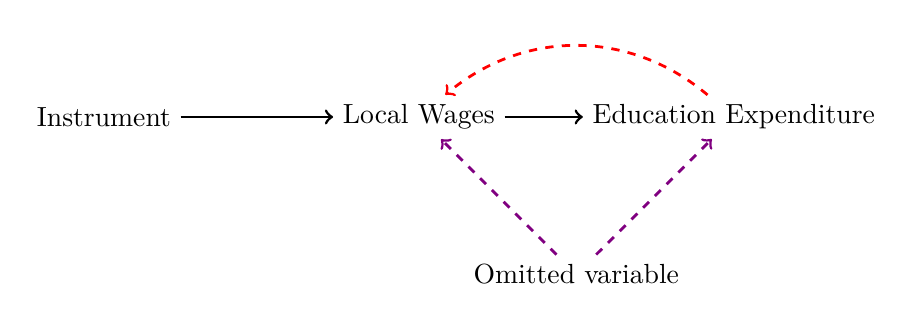
\begin{tikzpicture}
% nodes %
\node[rectangle] (z) at (0,0) {Instrument};
\node (t) at (4,0) {Local Wages};
\node (y) at (8,0) {Education Expenditure};
\node (u) at (6,-2) {Omitted variable};

% edges %
\draw[->, line width=1] (z) -- (t);
\draw[->, line width=1] (t) -- (y);
\draw[->, line width=1, violet, dashed] (u) -- (t);
\draw[->, line width=1, violet, dashed] (u) -- (y);
\draw[->, line width=1, red, bend right=40, dashed] (y) to (t);
\end{tikzpicture}
\label{fig:iv-approach}
\end{figure}

\subsubsection{Shift-share Instrument}\label{shift-share-instrument}

Therefore, we adopt a causal identification strategy via a shift-share
instrument. Shift-share or \emph{Bartik} instruments have gained
popularity in empirical work as a method of handling endogeneity issues
in panel data (\citet{ferri2022}, \citet{goldsmith-pinkham2020},
\citet{bartik1991}).\footnote{Autor et al.~use a shift-share instrument
  to assess the effect of Chinese import competition on manufacturing
  employment in US commuting zones (\citet{autor2013}). As an extension,
  \citet{feler2017} use a similar shift-share instrument to assess the
  effect of the same shock on the size of local government.
  \citet{baccini2021} employ a shift-share instrument for manufacturing
  layoffs to tease out the effect of a decline in manufacturing on both
  economically motivated and racial identity voting patterns in the US.}
Such instruments combine time-variant, unit-invariant changes in
aggregate economic variables (i.e., national changes in industry value
added levels) with time-invariant, unit-variant shares in exposure to
these macro-level changes (i.e., local shares of employment in
particular industries). This decomposition of local-level changes
delocalises variation over space and time. In doing so, it provides a
defensible strategy for `de-endogenising' the treatment, as local
exposure is predetermined with respect to contemporaneous shocks.
Moreover, by construction, the approach enables the examination of how
macro-level phenomena propagate to and affect local units, as it
generates local shocks that are driven by national industry trends
weighted but the community exposure to this industries.\footnote{An
  additional popular indicator for modelling industrial shocks is
  \emph{oil price} as values are often assumed to be exogenous to local
  and even national conditions (\citet{scheer2022}). Third, various
  indicators for measuring \emph{deindustrialisation} have been proposed
  including the manufacturing share of employment, value added, and GDP
  \citet{tregenna2009}, \citet{tregenna2020}. Finally, in rare
  instances, exogeneity can be secured due to \emph{geographical,
  climatological, or geological factors}. For example, \citet{borge2015}
  obtain an exogenous measure of local revenue by ``instrumenting the
  variation in hydropower revenue, and thus total revenue, by topology,
  average precipitation and meters of river in steep terrain.'' Certain
  authors have argued that the fact that the location of hydrocarbon
  deposits is dictated by geomorphological processes provides a
  plausible argument for exogeneity \citet{esposito2021},
  \citet{chen2022}.}

In the context of this work, we construct the instrument by interacting
commuting-zone level industrial employment shares held constant at a
base period with national real value added growth by industry. The
literature on Bartik instruments allows for an argument of plausible
exogeneity via various channels. First, authors argue that local
industry shares are exogenous by imposing that shares be fixed to a
particular base year and are therefore unable to adapt to changes in
national-level growth rates. Such a shift-share instrument is designed
as in Equation~\ref{eq-ref-bartik}.

\begin{equation}\phantomsection\label{eq-ref-bartik}{
Z_{it} = \sum_{j=1}^{k} S_{ij\tau}G_{njt}
}\end{equation}

where \(S_{ij\tau}\) is the local share of unit \(i\)'s economy
(measured using metrics like employment, wages, revenue) in industry
\(j\) at a fixed base year \(\tau\) and \(G_{njt}\) is the growth rate
of industry \(j\) at a national level \(n\) at time \(t\).

Alternatively, authors may argue that the claim of exogeneity in the
national-level growth rates is unlikely to be violated even when
allowing the local shares to vary over time. This approach is likely to
come at significant expense to instrument exogeneity. It is constructed
as follows:

\[
Z_{it} = \sum_{j=1}^{k} S_{ijt}G_{njt}
\]

Finally, authors might be concerned about the implausible exogeneity of
both shares and national-level growth rates in which case they construct
the instrument as in Equation~\ref{eq-ref-bartik-2} where the local
shares are fixed at a common base year and industry-specific growth
rates \(G\) are derived from data on other similar regions \(o\) rather
than national-level changes that are inherently comprised of local-level
shifts. This approach likely comes at significant expense to instrument
relevance.

\begin{equation}\phantomsection\label{eq-ref-bartik-2}{
Z_{it} = \sum_{j=1}^{k} S_{0jt}G_{ojt}
}\end{equation}

Finally, the authors can make an additional design choice about whether
the effect of these instruments should be assumed common to an aggregate
local-level wage growth indicator or allowed to vary by industry. In
other words, whether to construct the first-stage relationship of the
2SLS as\ldots:

\[
X_{it} = \alpha_i + \beta\sum_{j=1}^{k}S_{ijt}G_{njt} + \epsilon_{it}
\]

\ldots or\ldots:

\[
X_{it} = \alpha_i + \sum_{j=1}^{k}\beta_{j}S_{j}G_{jt} + \epsilon_{it}
\]

We employ the formulation in Equation~\ref{eq-ref-bartik}, assuming that
base-period local industry shares and time-varying national rates are
exogenous to local outcomes and construct the former of the first-stage
relationship assuming a common \(\beta\) to the sum of these shares.

Using data from the Bureau of Economic Analysis, we construct a
shift-share Bartik instrument at the commuting zone level using local
employment shares by industry and national changes in industry-specific
real value added represented in Equation~\ref{eq-bartik}. \(G_{njt}\)
represents national-level changes in value added in industry \(j\) in
time \(t\) and \(\frac{N_{ij\tau}}{N_{i\tau}}\) represents the
`sensitivity' of a CZ to these national shocks proxied by an initial
share of local employment in industry \(j\) in a baseline time period
\(\tau\). The product of these two values defines the shift-share
indicator \(\tilde{Z}_{i,t,s}\). In order to construct the share
portion, we compute the total local share of employment in a particular
industry \(j\). Due to challenges with missing data, we compute an
average share across 2001-2005 as our `base year'.

We compute the relevant shift-share instrument across 19 two-digit NAICS
industrial categories listed in \autoref{tbl_naics_codes}. Given
industry-level disaggregation of local employment data requires data
suppression for anonymity reasons, Figure 2 displays the data coverage
of our commuting zone level shift-share instruments. Given the high
degree of missingness in the 3-digit categorisation we proceed with the
2-digit NAICS codes.

In the Appendices, we provide an additional estimation using a
wage-based shift-share instrument constructed using data from the US
Bureau of Labor Statistics' Quarterly Census of Employment and Wages
(QCEW). This shift-share instrument is constructed as described above
using industry-level changes in real wages. Concerns about endogeneity
between the instrument and outcome variable are greater using this
shift-share instrument and is therefore excluded from the main text.
\footnote{We explore the sensitivity of results to the choice of base period
    $\tau$ by constructing the instrument for various base periods as
    well as a rolling window.}

\begin{equation}\phantomsection\label{eq-bartik}{
    \tilde{Z}_{it} = \sum_{j=1}^{k}G_{njt} *  \frac{N_{ij\tau}}{N_{i\tau}} 
}\end{equation}

\subsubsection{Empirical Estimation}\label{empirical-estimation}

This yields a 2SLS AR(1) model defined by the first- and second-stage
regressions represented in Equation~\ref{eq-first-stage} and
Equation~\ref{eq-second-stage}. Due to the likely presence of
time-dynamic effects, we include contemporaneous, 1-year, 2-year time
lags as instruments.

\begin{equation}\phantomsection\label{eq-first-stage}{
\textbf{(First stage)}\qquad
X_{it} \;=\; \rho\,X_{i,t-1} \;+\; \phi \,Y_{i,t-1} \;+\; \sum_{\ell=0}^{2}\pi_{\ell}\,\tilde Z_{i,t-\ell}
\;+\; \boldsymbol{\theta}\mathbf{W}_{it}' \;+\; \alpha_i \;+\; \lambda_t \;+\; u_{it},
}\end{equation}

\begin{equation}\phantomsection\label{eq-second-stage}{
\textbf{(Second stage)}\qquad
Y_{it} \;=\; \phi^\ast \,Y_{i,t-1} \;+\; \beta\,\widehat{X}_{it}
\;+\; \boldsymbol{\delta}\mathbf{W}_{it}'\;+\;  \alpha_i \;+\; \lambda_t \;+\; \varepsilon_{it}
}\end{equation}

where \(W_{it}\) is a vector of control variables. We control for
enrollment levels to account for scaling factors in education
expenditure, intergovernmental transfers to account for the significant
role of such transfers in funding education expenditure, percentage of
the population that is Black, percentage of the population that is
Hispanic, and private industry GDP per capita levels to account for
local price levels.

\(Y_{it}\) is the natural logarithm of elementary (serving ages 6-12)
education expenditure per pupil for CZ \(i\) in year \(t\). We focus on
elementary education for two reasons. First, this restriction partly
shields against a justifiable concern about the endogeneity between
wages and quality of local public education. Whereas funding for high
school could likely affect local wages given such students are of
working age, funding for elementary education is unlikely to impact wage
rates via a human capital or skills channel. Second, in terms of public
impact, elementary education is of foundational importance in the lives
of children. Slips in public education provision at a young age could
have scarring effects.

\(\alpha_i\) represents a CZ fixed effect and \(\lambda_t\) represents
year-fixed effects, with stage-relevant superscripts.
\(\varepsilon_{it}\) and \(u_{it}\) represents the error term of the
second and first stage, respectively.

We additionally adopt a dynamic specification by including lagged
dependent variables in both stages of the IV estimation to avoid
spurious correlation identification arising from persistence in
expenditure and wage levels, as well as better accounting for
heterogeneity across units. Education spending likely exhibits inertia
due to slowly evolving budgetary and relevant policy cycles (i.e.,
property tax rate setting). Similarly, local wage levels are
well-predicted by a previous year's wage levels. Failing to account for
these dynamics, our estimates would conflate the causal effect of wage
innovations with mechanical persistence in levels. This yields a more
conservative and interpretable elasticity, though we demonstrate that
the exclusion of the AR(1) term in the second-stage yields a
contemporaneous effect estimate nearly identical to the long-run wage
effect as derived from the dynamic specification in
\autoref{tbl_va_ss_baseline}.

\subsubsection{Interpretation}\label{interpretation}

The elasticity of public education expenditure to local wages has an
ambiguous interpretation. A positive elasticity would suggest that
higher wages increase household savings rates and willingness to invest
in local public goods, consistent with standard wealth effects. However,
this relationship raises concerns about possible divergence wherein wage
growth in high-earning regions could amplify educational investment,
potentially widening spatial inequality in public education quality
aligning with patterns of income inequality.

Conversely, a negative elasticity could emerge through several channels.
Any response in needs-based intergovernmental revenue mechanisms may
partially offset local fiscal capacity, creating an inverse relationship
between wages and education spending. Alternatively, in more affluent
communities, rising wages may enable households to substitute towards
private education, crowding out or reducing demand for public
expenditure. Furthermore, such a relationship could provide additional
empirical support for a ``resource curse'' dynamic\footnote{Perhaps the
  most prominent and often-cited relationship between education and
  extractive industries is through the lens of the `resource curse.' The
  validity and empirical existence of a `resource curse' has been tested
  since its conception with disparate results \citep[\citet{badeeb2017},
  \citet{blanco2012}, \citet{borge2015}, \citet{brunnschweiler2008},
  \citet{cockx2014}, \citet{cockx2016}, \citet{deacon2011},
  \citet{dialga2022}, \citet{douglas2017}, \citet{haber},
  \citet{menaldo2016}, \citet{ross2018}, \citet{ross2015},
  \citet{sincovich2018}, \citet{wiens2014}]{ahlerup2020}. The literature
  is divided into two strands focusing on either political (the
  relationship between resource wealth and governance)
  \citep[\citet{ross2015}, \citet{wiens2014},
  \citet{deacon2011}]{ross2015} or economic (the relationship between
  resource wealth and economic growth or human capital) resource curses.
  Empirical investigation of the economic resource curse has explored
  the effect of resource dependence on economic growth, public health
  and education expenditure and outcomes, mainly at a national level
  \citep[\citet{cockx2016}, \citet{douglas2017},
  \citet{sincovich2018}]{borge2015}. In the case of education, the
  distinct outcome measured is level of educational attainment, in other
  words, whether the presence of a booming resource extraction economy
  provides disincentives to education for young people. It is worth
  noting that this literature has been repeatedly questioned on
  theoretical and conceptual grounds as institutional context often
  dictates whether a resource curse exists and empirical analyses seem
  to be very sensitive to methodological choices
  \citep[\citet{ross2015}, \citet{dialga2022}]{ross2018}. Although
  awareness of this strand of literature is of relevance to this work,
  the unresolved nature of the `debate' surrounding its existence
  requires caution if eventually utilised as a theoretical framework for
  answering the research question. \citet{ahlerup2020} find that for 30
  countries in Africa, the presence of gold mines during adolescence
  have a significant effect on educational attainment.
  \citet{badeeb2017} investigates whether resource dependence slows
  economic growth with no explicit mention of education.
  \citet{blanco2012} find that in Latin America, petroleum export has a
  significant long-run negative relationships with human capital.
  \citet{borge2015} find support for the paradox of plenty hypothesis in
  Norway - that higher local public revenue negatively affects the
  efficiency of local public good provision. \citet{brunnschweiler2008}
  critically evaluate `the empirical basis for the so-called resource
  curse and find that, despite the topic's popularity in economics and
  political science research, this apparent paradox may be a red
  herring. The most commonly used measure of ``resource abundance'' can
  be more usefully interpreted as a proxy for ``resource
  dependence''-endogenous to underlying structural factors. In multiple
  estimations that combine resource abundance and dependence,
  institutional, and constitutional variables, we find that (i) resource
  abundance, constitutions, and institutions determine resource
  dependence, (ii) resource dependence does not affect growth, and (iii)
  resource abundance positively affects growth and institutional
  quality.' \citet{cockx2014} use a panel on 140 countries from
  1995-2009 and find an inverse relationship between resource dependence
  and and public health spending over time. \citet{cockx2016}
  investigate a panel of 140 countries from 1995-2009 to find an adverse
  effect of resource depdence on public education expenditures relative
  to GDP. \citet{dialga2022} find disparate results for health and
  education controlling for institutional quality. \citet{douglas2017}
  ``measure the effect of resource-sector dependence on long-run income
  growth using the natural experiment of coal mining in 409 Appalachian
  counties selected for homogeneity. Using a panel data set
  (1970--2010), we find a one standard deviation increase in resource
  dependence is associated with 0.5--1 percentage point long-run and a
  0.2 percentage point short-run decline in the annual growth rate of
  per capita personal income. We also measure the extent to which the
  resource curse operates through disincentives to education, and find
  significant effects, but this ``education channel'' explains less than
  15 percent of the apparent curse.' \citet{haber} focus on authoriarian
  regimes. \citet{menaldo2016} argues again that this is an institutions
  curse and not a resource curse issure. \citet{sincovich2018} provide a
  literature review of resource curse investigations in the Australian
  context.} wherein local communities reprioritise fiscal windfalls
toward government expenditure other than public education.

In either case, the consequence of a non-zero elasticity, whether
positive or negative, has potential adverse consequences for spatial
inequality of public education delivery by either boosting public
education in affluent areas or dampening investment in less affluent
areas.

Finally, a near-zero elasticity either has a modelling or
policy-relevant implication. On the modelling side, a near-zero
elasticity could indicate either that the wage-public goods relationship
operates on a longer time scale than that examined in this work. This
would indicate the need for an alternative identification strategy.
Alternatively, a near-zero elasticity could indicate that local public
education systems are effectively insulated from local wage changes
partly because intergovernmental transfers successfully equalise funding
across regions.

\subsubsection{Results}\label{results}

\FloatBarrier

\begin{table}[ht]
\centering
\begin{tabular}{ll}
  \hline
NAICS.Code & Industry \\ 
  \hline
11 & Agriculture, Forestry, Fishing, and Hunting \\ 
  21 & Mining \\ 
  23 & Construction \\ 
  31-33 & Manufacturing \\ 
  42 & Wholesale Trade \\ 
  44-45 & Retail Trade \\ 
  48-49 & Transportation and Warehousing \\ 
  22 & Utilities \\ 
  51 & Information \\ 
  52 & Finance and Insurance \\ 
  53 & Real Estate and Rental and Leasing \\ 
  54 & Professional, Scientific, and Technical Services \\ 
  55 & Management of Companies and Enterprises \\ 
  56 & Administrative and waste management services \\ 
  61 & Educational Services \\ 
  62 & Health Care and Social Assistance \\ 
  71 & Arts, Entertainment, and Recreation \\ 
  72 & Accommodation and Food Services \\ 
  81 & Other Services, except government \\ 
  92 & Public Administration \\ 
   \hline
\end{tabular}
\caption{Industry Categories} 
\label{tbl_naics_codes}
\end{table}

\begin{figure}[H]

{\centering \pandocbounded{\includegraphics[keepaspectratio]{regressions_files/figure-pdf/fig_wage_elasticity-1.png}}

}

\caption{Data Coverage of Industry-level Employment as Share of Total
Reported Employed}

\end{figure}%

In \autoref{tbl_va_ss_baseline}, we demonstrate a strong and highly
significant first-stage relationship wherein our shift-share instrument
indicates a strong positive contemporaneous relationship with local
wages. Our main specification in Columns 1-2 indicates that a 10\%
nicrease in local wages leads to a 2.23\% increase in per-pupil
education expenditure in the short run. The first-stage F-statistic
substantially exceeds conventional weak instrument thresholds. The
Wu-Hausman test definitevely rejects the exogeneity of wages, validating
our instrumental variable approach. However, the Wald
over-identification test suggests potential instrument invalidity,
though this is likely an artifact of the inclusion of AR(1) terms in the
first-stage and not an indictment of the exclusion restriction itself.
The implied long-run elasticity is near 0.46, indicating that the
cumulative effect of a 10\% wage increase is a 4.6\% increase in
education spending.

In Columns 3-4, we corroborate this long-run effect by removing the
AR(1) term in the second-stage regression. The statistically significant
causal effect of the treatment approaches this long-run effect of 4.6\%
(5.6\%), capturing the total association between wages and expenditures,
including both the immediate and long-run effects. This near-equivalence
in the estimated effect reflects the fact that the underlying
data-generating process is defined by dynamics, validating our use of a
fully dynamic system.

Understanding that wage shocks are likely transmitted to education
expenditure through property taxes, we test this potential mechanism in
columns 5-6 (adjusting the set of control variables to better suit the
first-stage relationship in theory). We find a highly significant house
price elasticity, wherein a 10\% increase in wages generate an 8.4\%
increase in local house prices. Note that the sample size decreases
because of missing data in the housing price index for several of our
commuting zones.

Our findings indicate that, in a decentralised education system, local
labour market strength affects public education expenditure. Regions
experiencing wage growth see spillovers into public education
expenditure, whereas communities facing wage stagnation or decline might
see their educational spending erode as a result.

\begin{table}[htbp]
   \caption{\label{tbl_va_ss_baseline} IV Estimation Using VA-based Shift-share instrument (l0, l1, l2) in Levels with CZ and year fixed effects and lags.}
   \centering
   \begin{adjustbox}{width = \textwidth, center}
      \begin{tabular}{lcccccc}
         \tabularnewline \midrule \midrule
         Dependent Variables:                                      & (log) Annual Avg. Wkly. Wage & (log) Elem.Ed.Exp.pp   & (log) Annual Avg. Wkly. Wage & (log) Elem.Ed.Exp.pp   & (log) Annual Avg. Wkly. Wage & (log) House Price Index\\  
         IV stages                                                 & First                        & Second                 & First                        & Second                 & First                        & Second \\   
         Model:                                                    & (1)                          & (2)                    & (3)                          & (4)                    & (5)                          & (6)\\  
         \midrule
         \emph{Variables}\\
         (log, l1) Annual Avg. Wkly. Wage                          & 0.7828$^{***}$               &                        & 0.7848$^{***}$               &                        & 0.7787$^{***}$               &   \\   
                                                                   & (0.0120)                     &                        & (0.0113)                     &                        & (0.0120)                     &   \\   
         VA SS (Lvl)                                               & -0.0179                      &                        & -0.0203                      &                        & 0.0257                       &   \\   
                                                                   & (0.0484)                     &                        & (0.0485)                     &                        & (0.0454)                     &   \\   
         VA SS (Lvl, l1)                                           & -0.1808$^{***}$              &                        & -0.1831$^{***}$              &                        & -0.1759$^{***}$              &   \\   
                                                                   & (0.0592)                     &                        & (0.0600)                     &                        & (0.0509)                     &   \\   
         VA SS (Lvl, l2)                                           & 0.1614$^{***}$               &                        & 0.1668$^{***}$               &                        & 0.1318$^{***}$               &   \\   
                                                                   & (0.0497)                     &                        & (0.0516)                     &                        & (0.0444)                     &   \\   
         (l1, log) Elem.Ed.Exp.pp                                  & 0.0039                       & 0.5086$^{***}$         &                              &                        &                              &   \\   
                                                                   & (0.0041)                     & (0.0156)               &                              &                        &                              &   \\   
         (log) IG Revenue pp                                       & 0.0135$^{***}$               & 0.2230$^{***}$         & 0.0143$^{***}$               & 0.3213$^{***}$         &                              &   \\   
                                                                   & (0.0030)                     & (0.0211)               & (0.0028)                     & (0.0316)               &                              &   \\   
         (log) Real GDP Priv. Industry pc                          & 0.0390$^{***}$               & 0.0662$^{***}$         & 0.0394$^{***}$               & 0.0946$^{***}$         & 0.0403$^{***}$               & 0.0381$^{***}$\\   
                                                                   & (0.0044)                     & (0.0144)               & (0.0044)                     & (0.0243)               & (0.0060)                     & (0.0083)\\   
         (log) Enrollment                                          & 0.0109$^{**}$                & -0.1957$^{***}$        & 0.0099$^{**}$                & -0.3306$^{***}$        &                              &   \\   
                                                                   & (0.0044)                     & (0.0157)               & (0.0042)                     & (0.0282)               &                              &   \\   
         \% Black                                                  & -0.1685$^{**}$               & 0.3333$^{*}$           & -0.1668$^{**}$               & 0.6541$^{*}$           & -0.0916                      & -0.4356$^{***}$\\   
                                                                   & (0.0724)                     & (0.1924)               & (0.0720)                     & (0.3622)               & (0.0745)                     & (0.1586)\\   
         \% Hispanic                                               & -0.0526                      & 0.0483                 & -0.0529                      & 0.0381                 & -0.0433                      & -0.0217\\   
                                                                   & (0.0327)                     & (0.1509)               & (0.0326)                     & (0.2516)               & (0.0345)                     & (0.0594)\\   
         (log) Annual Avg. Wkly. Wage                              &                              & 0.2269$^{***}$         &                              & 0.5618$^{***}$         &                              & 0.0873$^{**}$\\   
                                                                   &                              & (0.0477)               &                              & (0.0765)               &                              & (0.0404)\\   
         (log, l1) House Price Index                               &                              &                        &                              &                        & 0.0142$^{***}$               & 0.8378$^{***}$\\   
                                                                   &                              &                        &                              &                        & (0.0049)                     & (0.0098)\\   
         \midrule
         \emph{Fixed-effects}\\
         unit                                                      & Yes                          & Yes                    & Yes                          & Yes                    & Yes                          & Yes\\  
         year                                                      & Yes                          & Yes                    & Yes                          & Yes                    & Yes                          & Yes\\  
         \midrule
         \emph{Fit statistics}\\
         Observations                                              & 12,084                       & 12,084                 & 12,084                       & 12,084                 & 11,509                       & 11,509\\  
         R$^2$                                                     & 0.99247                      & 0.90636                & 0.99247                      & 0.86539                & 0.99337                      & 0.99074\\  
         Within R$^2$                                              & 0.77623                      & 0.51804                & 0.77617                      & 0.30715                & 0.78832                      & 0.78569\\  
         Wu-Hausman                                                &                              & 44.905                 &                              & 138.75                 &                              & 115.32\\  
         Wu-Hausman, p-value                                       &                              & $2.17\times 10^{-11}$  &                              & $7.64\times 10^{-32}$  &                              & $9.12\times 10^{-27}$\\   
         Wald (IV only)                                            & 1,345.2                      & 22.645                 & 1,517.9                      & 53.948                 & 1,103.7                      & 4.6738\\  
         Wald (IV only), p-value                                   & $0\times 10^{-16}$           & $1.97\times 10^{-6}$   & $0\times 10^{-16}$           & $2.19\times 10^{-13}$  & $0\times 10^{-16}$           & 0.03065\\  
         F-test (1st stage)                                        & 5,972.4                      &                        & 6,261.7                      &                        & 5,008.7                      & \\  
         F-test (1st stage), (log) Annual Avg. Wkly. Wage          &                              & 5,972.4                &                              & 6,261.7                &                              & 5,008.7\\  
         F-test (1st stage), p-value                               & $0\times 10^{-16}$           &                        & $0\times 10^{-16}$           &                        & $0\times 10^{-16}$           & \\  
         F-test (1st stage), p-value, (log) Annual Avg. Wkly. Wage &                              & $0\times 10^{-16}$     &                              & $0\times 10^{-16}$     &                              & $0\times 10^{-16}$\\   
         \midrule \midrule
         \multicolumn{7}{l}{\emph{Clustered (unit) standard-errors in parentheses}}\\
         \multicolumn{7}{l}{\emph{Signif. Codes: ***: 0.01, **: 0.05, *: 0.1}}\\
      \end{tabular}
   \end{adjustbox}
\end{table}

\FloatBarrier

\subsection{Accounting for
Heterogeneity}\label{accounting-for-heterogeneity}

In order to make meaningful policy-related insights, we need to unmask
the substantial heterogeneity obscured by national-level average
treatment effects. These national-level estimates are unlikely to apply
uniformly across states and commuting zones, especially given
heterogeneity in local tax regimes.

Therefore, we (1) use data on local wages and GDP to create indicators
for whether regions are exhibiting relative decline or growth compared
to other commuting zones to partition our sample in a data-driven
manner, employ (2) industry-by-industry and (2) state-by-state
estimations in our IV specifications using our VA-based shift-share
instrument.

For completeness, we provide results of average treatment effects for
all implemented estimations in the Appendices.

\subsubsection{Declining vs.~Growing Regions}\label{sec-growthrates}

First, we identify declining and growing regions by estimating
commuting-zone wage and private industry GDP growth rates conditional on
state and national level growth rates and partition our sample across
this distribution.

In order to identify declining and growing commuting zones, we estimate
separate time series models by commuting zone as follows. These models
allow for the identification of commuting-zone level growth rates while
controlling for state and national trends in a two-step framework.
First, we orthogonalize the state-level growth rate with respect to the
national trend, isolating state-specific fluctuations unrelated to the
national business cycle:

\[
\widetilde{\Delta \log GDPpc}^{state}_{t} 
= \Delta \log GDPpc^{state}_{t} 
- \hat{\gamma}\, \Delta \log GDPpc^{nat}_{t}
\] Second, we regress commuting zone growth on both the national growth
rate and the orthogonalized state residuals, thereby decomposing local
growth into national, state, and idiosyncratic components. This approach
identifies commuting zones whose trajectories systematically diverge
from higher-level aggregate patterns, providing a clean measure of
relative local economic performance.

\[
\Delta \log GDPpc^{CZ}_{t} 
= \alpha_{g} 
+ \beta_{n} \, \Delta \log GDPpc^{nat}_{t} 
+ \beta_{s} \, \widetilde{\Delta \log GDPpc}^{state}_{t} 
+ \varepsilon_{t}
\]

In these equations, each GDP term represents the private industry GDP
per capita at the CZ, state, or national level, denoted by superscript.

Intuitively, this specification measures how much of each CZ's growth
can be explained by broader aggregate trends versus localized factors.
By controlling for orthogonalized state and national variation, the
estimated intercept (\(\alpha_{g}\)) and residual terms capture
persistent, region‐specific trends that are not driven by common
macroeconomic forces. This allows us to identify which commuting zones
are systematically growing or declining relative to their state and
national baselines, thereby providing a purer measure of local economic
dynamics that is robust to shared higher-level
shocks.\footnote{We provide similar analysis of gross GDP in the Appendix.}

We perform the same trend deviation calculation for wages where each
wage variable represents the commuting zone, state, and national level
growth rate in the weekly average wage as reported in QCEW.

\[
\widetilde{\Delta \log Wage}^{state}_{t} 
= \Delta \log Wage^{state}_{t} 
- \hat{\gamma}\, \Delta \log Wage^{nat}_{t}
\]

\[
\Delta \log Wage^{CZ}_{t} 
= \alpha_{w} 
+ \beta_{n} \, \Delta \log Wage^{nat}_{t} 
+ \beta_{s} \, \widetilde{\Delta \log Wage}^{state}_{t} 
+ \varepsilon_{t}
\]

Figure 5 plots the distribution of values of \(\alpha_g\), \(\alpha_w\),
and the distribution of commuting-zone level loadings on national and
state-level growth rates. The figure demonstrates that commuting zones
load more variably onto state-level growth rates and more consistently
onto national-level growth rates. These distributions are expected by
design as the state-level growth rates provide variation that the
national level rates do not.

Next, Figure 6 demonstrates the considerable variability in GDP-level
growth rates across commuting zones in the US between 2001-2021.
Visualising the per capita growth rate deviations by state and region
demonstrates heterogeneity in this variability across states and
regions. For example, Texas, Montana, North Dakota, and Colorado have
outstanding positive outliers in the distribution whereas Kentucky,
Louisiana, South Dakota have outstanding negative outliers. The grey
lines represent the commuting zones value of \(\alpha_w\), indicating
that in a large share of cases, wage growth rates are defined by a
different sign than the GDP growth rates, indicating even potential
local divergence in growth rates. Though the calculations above could
lead to insignificant such relationships because the growth rates are
calculated in reference to different data, the volume of states
exhibiting diverging wage and GDP per capita growth rates indicate that
such a divergence is likely a fact of life in many commuting zones.

To account for this inherent incomparability of the growth rates
\(\alpha_w\) and \(\alpha_g\), we display a standard Pearson correlation
coefficient between teh commuting zone time series of GDP per capita and
wages, indicating that several states house commuting zones whose wages
do not track GDP growth. Many states see nearly exclusively positive
correlation coefficients, whereas others see a mix of commuting zones
where the relationship is positive or negative.

\begin{figure}[H]

{\centering \pandocbounded{\includegraphics[keepaspectratio]{regressions_files/figure-pdf/wage_gdp_trend-1.png}}

}

\caption{GDPpc and Wage Growth Rates and Loadings}

\end{figure}%

\begin{figure}[H]

{\centering \pandocbounded{\includegraphics[keepaspectratio]{regressions_files/figure-pdf/wage_gdp_trend-2.png}}

}

\caption{Lollipop Plot of Wage and GDPpc Growth Rates}

\end{figure}%

\begin{figure}[H]

{\centering \pandocbounded{\includegraphics[keepaspectratio]{regressions_files/figure-pdf/unnamed-chunk-19-1.png}}

}

\caption{Correlation Between GDP Growth Rates and Wage Growth Rates by
State}

\end{figure}%

\paragraph{Sample Partitioning by Growth
Rates}\label{sample-partitioning-by-growth-rates}

Using these growth rates, we partition the sample according to the
percentiles described above. \autoref{tbl_gdp_ss_wage_subsamples} and
\autoref{tbl_gdp_ss_gdp_subsamples} examine how the relationship between
local economic conditions and elementary education expenditure per pupil
varies across structurally growing and declining regions as defined in
the previous section. We partition our sample into four sub-samples by
their values of \(\alpha_{w}\) and \(\alpha_{g}\) as shown in
Table~\ref{tbl-categories}.

\begin{longtable}[]{@{}ll@{}}
\caption{Category Definitions}\label{tbl-categories}\tabularnewline
\toprule\noalign{}
Category & Definition (\(\alpha_{w}\), \(\alpha_{g}\)) \\
\midrule\noalign{}
\endfirsthead
\toprule\noalign{}
Category & Definition (\(\alpha_{w}\), \(\alpha_{g}\)) \\
\midrule\noalign{}
\endhead
\bottomrule\noalign{}
\endlastfoot
Declining & \(\alpha < 0\) \\
Hyper-Declining & \(\alpha < P_{25}\) \\
Growing & \(\alpha > 0\) \\
Hyper-Growing & \(\alpha > P_{75}\) \\
\end{longtable}

Zones with negative (positive) values of \(\alpha_{w}\) or \(\alpha_g\)
are designated as declining (growing), while those in the bottom (P25)
and top (P75) quartiles are labelled hyper-declining and hyper-growing,
respectively. This stratification enables comparison of fiscal
responsiveness across local economies with different long-run growth
trajectories.

\autoref{tbl_gdp_ss_wage_subsamples} partitions CZs by \(\alpha_w\).
Interestingly, we observe positive statistically significant
relationships between wages and public education expenditure though the
magnitude and statistical significance of this relationship declines
almost uniformly as \(\alpha_w\) discretely increases. We see a similar
declining size and significance in the explanatory variable accounting
for inter-governmental revenue, indicating that these revenues play a
smaller role in regions exhibiting above-average wage growth.

In \autoref{tbl_gdp_ss_gdp_subsamples} partitions CZs by long-run GDP
per capita trends. The statistical significance and magnitude variations
in the wage response tell a less monotonic story here, likely mirroring
the lack of systematic correlation between \(\alpha_w\) and \(\alpha_g\)
When partitioning the sample by GDP growth rates, the interpretation is
more straight-forward.

Regardless, all models remain well-identified, with high first stage F
statistics, convincing performance on the Wu-Hausman endogeneity tests
and Wald tests. Combined, these results indicate that partitioning by
background wage growth rates provides greater insight into the sample's
heterogeneity than diversity in GDP per capita growth rates. More
precisely, given communities feel wage growth more directly than GDP per
capita improvements, it is likely that the relationship between public
education and wage changes is better captured by sub-sampling by wage
growth rates.

\FloatBarrier

\FloatBarrier

\begin{table}[htbp]
   \caption{\label{tbl_gdp_ss_wage_subsamples} Second-Stage: VA-based Shift-Share Instrument (l1) Applied to Declining Wage vs. Growing Wage Regions}
   \centering
   \begin{adjustbox}{width = \textwidth, center}
      \begin{tabular}{lccccc}
         \tabularnewline \midrule \midrule
         Dependent Variable: & \multicolumn{5}{c}{(log) Elem.Ed.Exp.pp}\\
                                                                   & All                    & Hyper-Declining (Wage) & Declining (Wage)      & Growing (Wage)        & Hyper-Growing (Wage) \\   
         Model:                                                    & (1)                    & (2)                    & (3)                   & (4)                   & (5)\\  
         \midrule
         \emph{Variables}\\
         (log) Annual Avg. Wkly. Wage                              & 0.2269$^{***}$         & 0.3277$^{***}$         & 0.3394$^{***}$        & 0.2128$^{***}$        & 0.1551$^{*}$\\   
                                                                   & (0.0477)               & (0.0683)               & (0.0861)              & (0.0527)              & (0.0830)\\   
         (l1, log) Elem.Ed.Exp.pp                                  & 0.5086$^{***}$         & 0.5148$^{***}$         & 0.5543$^{***}$        & 0.5019$^{***}$        & 0.5311$^{***}$\\   
                                                                   & (0.0156)               & (0.0267)               & (0.0332)              & (0.0173)              & (0.0290)\\   
         (log) IG Revenue pp                                       & 0.2230$^{***}$         & 0.2800$^{***}$         & 0.2101$^{***}$        & 0.2245$^{***}$        & 0.1553$^{***}$\\   
                                                                   & (0.0211)               & (0.0341)               & (0.0317)              & (0.0239)              & (0.0391)\\   
         (log) Real GDP Priv. Industry pc                          & 0.0662$^{***}$         & 0.0156                 & 0.0220                & 0.0703$^{***}$        & 0.0685$^{***}$\\   
                                                                   & (0.0144)               & (0.0238)               & (0.0313)              & (0.0150)              & (0.0160)\\   
         (log) Enrollment                                          & -0.1957$^{***}$        & -0.2269$^{***}$        & -0.1995$^{***}$       & -0.1941$^{***}$       & -0.2001$^{***}$\\   
                                                                   & (0.0157)               & (0.0254)               & (0.0351)              & (0.0175)              & (0.0332)\\   
         \% Black                                                  & 0.3333$^{*}$           & 0.2172                 & 0.2137                & 0.3892$^{*}$          & 1.193$^{**}$\\   
                                                                   & (0.1924)               & (0.2664)               & (0.3680)              & (0.2294)              & (0.5557)\\   
         \% Hispanic                                               & 0.0483                 & 0.2597                 & 0.2509                & 0.0110                & 0.1335\\   
                                                                   & (0.1509)               & (0.2566)               & (0.1897)              & (0.1781)              & (0.3037)\\   
         \midrule
         \emph{Fixed-effects}\\
         unit                                                      & Yes                    & Yes                    & Yes                   & Yes                   & Yes\\  
         year                                                      & Yes                    & Yes                    & Yes                   & Yes                   & Yes\\  
         \midrule
         \emph{Fit statistics}\\
         Observations                                              & 12,084                 & 3,021                  & 1,520                 & 10,564                & 3,021\\  
         R$^2$                                                     & 0.90636                & 0.92102                & 0.94210               & 0.89805               & 0.90098\\  
         Within R$^2$                                              & 0.51804                & 0.57170                & 0.58942               & 0.50752               & 0.50064\\  
         Wu-Hausman                                                & 44.905                 & 12.495                 & 8.9646                & 36.833                & 18.989\\  
         Wu-Hausman, p-value                                       & $2.17\times 10^{-11}$  & 0.00041                & 0.00280               & $1.33\times 10^{-9}$  & $1.36\times 10^{-5}$\\   
         Wald (IV only)                                            & 22.645                 & 23.023                 & 15.549                & 16.276                & 3.4973\\  
         Wald (IV only), p-value                                   & $1.97\times 10^{-6}$   & $1.68\times 10^{-6}$   & $8.41\times 10^{-5}$  & $5.52\times 10^{-5}$  & 0.06157\\  
         F-test (1st stage), (log) Annual Avg. Wkly. Wage          & 5,972.4                & 1,354.5                & 813.43                & 5,156.1               & 1,214.4\\  
         F-test (1st stage), p-value, (log) Annual Avg. Wkly. Wage & $0\times 10^{-16}$     & $0\times 10^{-16}$     & $0\times 10^{-16}$    & $0\times 10^{-16}$    & $0\times 10^{-16}$\\   
         \midrule \midrule
         \multicolumn{6}{l}{\emph{Clustered (unit) standard-errors in parentheses}}\\
         \multicolumn{6}{l}{\emph{Signif. Codes: ***: 0.01, **: 0.05, *: 0.1}}\\
      \end{tabular}
   \end{adjustbox}
\end{table}
\begin{table}[htbp]
   \caption{\label{tbl_gdp_ss_gdp_subsamples} Second-Stage: VA-based Shift-Share Instrument (l1) Applied to Declining GDP vs. Growing GDP Regions}
   \centering
   \begin{adjustbox}{width = \textwidth, center}
      \begin{tabular}{lccccc}
         \tabularnewline \midrule \midrule
         Dependent Variable: & \multicolumn{5}{c}{(log) Elem.Ed.Exp.pp}\\
                                                                   & All                    & Hyper-Declining (GDP) & Declining (GDP)       & Growing (GDP)         & Hyper-Growing (GDP) \\   
         Model:                                                    & (1)                    & (2)                   & (3)                   & (4)                   & (5)\\  
         \midrule
         \emph{Variables}\\
         (log) Annual Avg. Wkly. Wage                              & 0.2269$^{***}$         & 0.2785$^{***}$        & 0.2912$^{***}$        & 0.1874$^{***}$        & 0.2532$^{***}$\\   
                                                                   & (0.0477)               & (0.0737)              & (0.0648)              & (0.0595)              & (0.0822)\\   
         (l1, log) Elem.Ed.Exp.pp                                  & 0.5086$^{***}$         & 0.5430$^{***}$        & 0.5286$^{***}$        & 0.4937$^{***}$        & 0.4893$^{***}$\\   
                                                                   & (0.0156)               & (0.0212)              & (0.0193)              & (0.0218)              & (0.0282)\\   
         (log) IG Revenue pp                                       & 0.2230$^{***}$         & 0.2290$^{***}$        & 0.2575$^{***}$        & 0.2086$^{***}$        & 0.1911$^{***}$\\   
                                                                   & (0.0211)               & (0.0405)              & (0.0345)              & (0.0275)              & (0.0397)\\   
         (log) Real GDP Priv. Industry pc                          & 0.0662$^{***}$         & 0.0378                & 0.0398                & 0.0714$^{***}$        & 0.0759$^{***}$\\   
                                                                   & (0.0144)               & (0.0358)              & (0.0320)              & (0.0160)              & (0.0172)\\   
         (log) Enrollment                                          & -0.1957$^{***}$        & -0.2011$^{***}$       & -0.1911$^{***}$       & -0.2017$^{***}$       & -0.2353$^{***}$\\   
                                                                   & (0.0157)               & (0.0332)              & (0.0238)              & (0.0209)              & (0.0295)\\   
         \% Black                                                  & 0.3333$^{*}$           & 0.1517                & 0.1511                & 0.6266$^{*}$          & 0.7367\\   
                                                                   & (0.1924)               & (0.2226)              & (0.1964)              & (0.3421)              & (0.7621)\\   
         \% Hispanic                                               & 0.0483                 & -0.1417               & -0.0061               & 0.0687                & -0.0070\\   
                                                                   & (0.1509)               & (0.2286)              & (0.1702)              & (0.1938)              & (0.2165)\\   
         \midrule
         \emph{Fixed-effects}\\
         unit                                                      & Yes                    & Yes                   & Yes                   & Yes                   & Yes\\  
         year                                                      & Yes                    & Yes                   & Yes                   & Yes                   & Yes\\  
         \midrule
         \emph{Fit statistics}\\
         Observations                                              & 12,084                 & 3,021                 & 5,016                 & 7,068                 & 3,021\\  
         R$^2$                                                     & 0.90636                & 0.90369               & 0.90765               & 0.90377               & 0.85786\\  
         Within R$^2$                                              & 0.51804                & 0.54248               & 0.55592               & 0.47980               & 0.48120\\  
         Wu-Hausman                                                & 44.905                 & 10.070                & 18.286                & 20.577                & 22.401\\  
         Wu-Hausman, p-value                                       & $2.17\times 10^{-11}$  & 0.00152               & $1.94\times 10^{-5}$  & $5.83\times 10^{-6}$  & $2.32\times 10^{-6}$\\   
         Wald (IV only)                                            & 22.645                 & 14.299                & 20.216                & 9.9366                & 9.5022\\  
         Wald (IV only), p-value                                   & $1.97\times 10^{-6}$   & 0.00016               & $7.07\times 10^{-6}$  & 0.00163               & 0.00207\\  
         F-test (1st stage), (log) Annual Avg. Wkly. Wage          & 5,972.4                & 1,846.6               & 2,651.0               & 3,287.8               & 1,501.4\\  
         F-test (1st stage), p-value, (log) Annual Avg. Wkly. Wage & $0\times 10^{-16}$     & $0\times 10^{-16}$    & $0\times 10^{-16}$    & $0\times 10^{-16}$    & $0\times 10^{-16}$\\   
         \midrule \midrule
         \multicolumn{6}{l}{\emph{Clustered (unit) standard-errors in parentheses}}\\
         \multicolumn{6}{l}{\emph{Signif. Codes: ***: 0.01, **: 0.05, *: 0.1}}\\
      \end{tabular}
   \end{adjustbox}
\end{table}

\FloatBarrier

\subsubsection{State-by-state
estimation}\label{state-by-state-estimation}

Next, given the substantial heterogeneity in state-level economic makeup
and public finance regimes, we investigate state-specific relationships
between our variables of interest.

First, states vary in the number of commuting zones they contain. Figure
12 demonstrates that states have anywhere between 2 (Delaware) and 58
(Texas) commuting zones. This allows us to estimate panel-style
regressions within each state to net out between-state variation that
might be confounding our current treatment estimates.

\begin{figure}[H]

{\centering \pandocbounded{\includegraphics[keepaspectratio]{regressions_files/figure-pdf/unnamed-chunk-26-1.png}}

}

\caption{Histogram: Commuting Zones by State}

\end{figure}%

\FloatBarrier

\FloatBarrier

Using our instrumental variable approach with a value-added based
shift-share instrument, we corroborate the directionality and magnitude
of the effect for 12 states: New Hampshire, Colorado, Florida, South
Dakota, Kentucky, Louisiana, Pennsylvania, North Dakota, Oregon,
Oklahoma, Arizona, and Indiana. In estimating the state-by-state
regressions, we exclude any states where our F-statistic is below
conventional weak instrument thresholds (F statistics \textless= 12 and
p-value \textless{} 0.05) and the p-value of the second stage
coefficient of interest is \textless{} 0.1.

Examining various characteristics of these states, we find that they
vary widely in demographic composition, enrollment levels, and wage
levels indicating that the detected effects are not attributable to any
extremes in these values. Notably, majority of them reuly on a
significant share of educational expenditure from local sources rather
than intergovernmental sources.

\begin{figure}[H]

{\centering \pandocbounded{\includegraphics[keepaspectratio]{regressions_files/figure-pdf/unnamed-chunk-28-1.png}}

}

\caption{State-by-State Wage Effect Using SS GDP Shock}

\end{figure}%

\subsubsection{Industry by Industry}\label{industry-by-industry}

Finally, given our shift-share instruments are the composite effect of
shifts in industry-level real value added (VA), we can decompose this
instrument into industry-specific real value added shocks. This
decomposition allows us to examine the effect of industry-specific
changes across states in a more explicit manner. In other words, we
re-design our instrument as\ldots{}

\begin{equation}\phantomsection\label{eq-bartik-decomposed}{
    \tilde{Z}_{ijt} = G_{njt} *  \frac{N_{ij\tau}}{N_{i\tau}}
}\end{equation}

\ldots rather than the sum of all industry-level shocks.

We estimate separate panel regressions using the full commuting zone
sample and then grouping commuting zones by state instrumenting local
level wages by these decomposed shift-share shocks by industry.

Using our value added-based shift share instrument, Figure 10
demonstrates the overall treatment effect of local wage changes
instrumented via an industry-specific GDP shock. We find that regardless
of the instrument design, the coefficient estimate is consistent with
the baseline results, where the estimated effect of a 10\% change to
local wages on public education expenditure is a 2.2\% increase, with
the effect's magnitude varying meaningfully for several states. We plot
the relevant state-level effects for those states whose estimations pass
the same restriction criteria as above (F statistics \textless= 12 and
p-value \textless{} 0.05 and the p-value of the second stage coefficient
of interest is \textless{} 0.1).

\textcolor{red}{Again, I want to improve this.}

\begin{figure}[H]

{\centering \pandocbounded{\includegraphics[keepaspectratio]{regressions_files/figure-pdf/indind-1.png}}

}

\caption{Wage Effect via Industry VA SS Shock}

\end{figure}%

\FloatBarrier

\subsection{Additional Analysis
Inventory}\label{additional-analysis-inventory}

In the Appendices we include:

\begin{itemize}
  \item Panel VAR Estimation
  \item Quantile regression estimation
  \item Exclusion of high-income CZ outliers
  \item Implementation of a wage-based (rather than VA-based) shift-share instrument
  \item National average treatment effects for all econometric estimation strategies outlined in the main text
  \item Information about the construction of the shift-share instrument
\end{itemize}

\FloatBarrier

\section{Conclusion}\label{conclusion}

\subsection{Discussion}\label{discussion}

This work establishes a causal link between local wage growth and public
education expenditure. Our baseline estimates reveal a short-run wage
elasticity of 0.23, with a long-run cumulative effect of approximately
0.46. The dynamic components of the econometric specification indicate
significant persistence in local public education budgets, indicating
both institutional inertia but also the likely rare revision of local
tax rates allowing local wage growth to boost education spending. This
persistence indicates potential for asymmetric adjustment likely
correlated with local growth trajectories, wherein communities
experiencing wage growth are likely to see gradual spending increases,
while declining communities could experience the opposite effect.

This positive elasticity is concentrated in a third of the states in the
sample (New Hampshire, Colorado, Florida, South Dakota, Kentucky,
Louisiana, Pennsylvania, North Dakota, Oregon, Oklahoma, Arizona, and
India), whereas other states exhibit minimal or insignificant
responsiveness.

Though outcomes measured in this study are not direct inequality
metrics, our findings reveal that the decentralised school financing
system in the US has the potential to exacerbate inequalities in local
public well-being by failing to equalise across regions experiencing
diverging growth trajectories. As a result, in the states in which local
spending is responsive to changes in local wages, the quality of early
childhood education might be compromised by macroeconomic trends and
industry-specific shocks beyond local control. Thus, equalisation
formulas at the state and federal level that fail to account for wage
trends and fiscal multipliers may contribute to disparities in public
goods delivery. Theories of effective equalisation, and indeed
preferences for redistribution, differ especially across regions of the
the United States. However, equalisation efforts should at least aim to
insulate communities from potential downward pressures on public
education expenditure.

The determinants of inequality in public education delivery in the US
are multiple and complex. Significant evidence exists of the role of
historically discriminatory policies related to congressional
districting, under-investment in low-income areas of color
\citet{trounstine2016} \citet{trounstine2021} \citet{sosina2019} .
Though this work does not directly inform this debate, further work
could explore the extent to which wage growth interacts with such
structural policies.

Addressing structural inequality requires rethinking education finance,
taking the decentralised American context as given. Ensuring educational
equity for all children requires not just strengthening existing
mechanisms for redistribution, but also, in light of our results,
insulating communities from macroeconomic trends that impact communities
heterogeneously.

\subsection{Limitations}\label{limitations}

\begin{itemize}
\item
  Excludability assumptions about local industry composition
\item
  Data limits true consideration of non-stationarity issues. Estimating
  this model in first differences or growth rates would be preferable to
  address non-stationarity concerns as well as allow for asymmetric
  treatmetn estimation to distinguish between negative and positive wage
  pressures. However, this would require improvements in data collection
  of the required variables.
\item
  Commuting zones mask substantial within-commuting zone heterogeneity
\end{itemize}

\section{Data and Code Availability}\label{data-and-code-availability}

\textcolor{red}{Code and data to reproduce the analysis will be made available on Github or Zenodo.}

\section{Use of AI}\label{use-of-ai}

\begin{itemize}
\tightlist
\item
  Used ChatGPT to help improve readability of plots (formatting,
  margins, labeling, font size).
\item
  Used ChatGPT to debug errors in R during data cleaning and plotting.
\item
  Used ChatGPT to provide suggestions for reducing run time of
  repetitive tasks (ex. downloading and processing multiple data files).
\end{itemize}

\section{Acknowledgements}\label{acknowledgements}

\section*{Appendices}\label{appendices}
\addcontentsline{toc}{section}{Appendices}

\appendix



\section{Modelling Challenges}
\label{si_section:Challenges}
Below, I provide a brief discussion of anticipated methodological challenges and constraints.

\subsection{Structure of Financing for Local Public Education}
\textbf{In order to appropriately make use of the outlined data as well as robustly define the econometric methods to be utilised in this work, an understanding of the funding structure of public school districts in the US is critical.} Public school districts in the United States are funded by a combination of federal (8.3\% in 2019), state (47\% in 2019), and local (44.8\% in 2019) revenues \cite{skinner2019}, with shares varying by county. This variation in public funding structure will need to be incorporated into the modelling efforts, likely through a weighted regression approach based on shares of intergovernmental versus own-source revenues \cite{skinner2019}. Using the data outlined, Figure \ref{fig:natl_share_rev} displays the share of public education revenue coming from three sources of intergovernmental revenue (federal, state, and local) as well as revenue from own county-level sources by state. The figure demonstrates the clear near-even split between state intergovernmental and own source revenue and the overall small share of revenue coming from federal or other local governments. The larger panel on the top left provides the summarising share at the national level. All plots share the axes as labeled in the top left panel.

\subsection{Trends over time}
According to the most recent data available from the US Congressional Research Service, the revenue share has shifted from local to state sources whereas federal funding has remained the same albeit with fluctuations over time \cite{skinner2019}.
\begin{figure}[ht]
    \caption{Share of Revenue from Federal, State, Local Sources \\
    }
    \centering
    \includegraphics[scale = 0.15]{../output/natl_shares_of_revenue_by_source.jpg}
    \label{fig:natl_share_rev}
\end{figure}
\FloatBarrier

\subsection{Historical efforts to ``equalise'' US public education}
\textbf{Another factor that greatly impacts the data generating process in this study is that increasing recognition of the level of inequality of public education provision in the US has led to the implementation of several efforts to ``equalise'' public education by aiming for "per pupil" expenditure targets \cite{skinner2019}.} The most significant change in this respect has been the creation of Educational Service Agencies (ESAs). These ESAs are apportioned state funding to serve multiple school districts in sub-regions of each state. Most of these ESAs were established around 2007 and persist to this day. ESAs are listed by state in Table \ref{tab:si_tbl:esa_names_tbl}. Currently, there are 553 agencies nationwide in 45 states. According to the Association of Educational Service Agencies (AESA), ESAs reach over 80\% of the public school districts and well over 80\% of public and private school students. Annual budgets for ESAs total approximately \$15 billion \cite{aesa2024}. Because ESA revenue and expenditure is inconsistently reported across years in our dataset, as well as attributed to individual counties despite often serving multiple, there is a significant risk that ESA expenditure is misattributed to counties in our dataset. Therefore, I exclude ESA revenue and expenditure totals from the measures of county-level expenditure and revenue at all levels of aggregation, and retain these values as possible control variables.

Preliminary investigation, both descriptive and using regression models, indicate that public expenditure from ESAs have not acted as a substitute for other revenue sources. In other words, they have not displaced intergovernmental or local school revenue. Although this fact ensures that changes in public spending on education detected in our models are not overestimated due to substitution effects from unmodelled ESA expenditure, it does risk underestimating values of actual expenditure per pupil. This remains to be resolved.

\subsection{Availability of varying local-level outcomes}

\textbf{Approaching a more "local" analysis of such challenges is often inhibited by data availability.} First, data limitations including infrequent periodicity and missingness due to strained local reporting capacity or low stringency impose a limit on the statistical power in a panel analysis. Furthermore, infrequent periodicity poses the additional challenge to interpretation when assessing the impact of industrial changes that are often subject to within-year cyclicality. 

\subsection{Structural and policy heterogeneity}

\textbf{County-level analysis of the US poses an inherent trade-off between greater local insight and requisite model complexity.} First, county-level variables are subject to unit- and time-dependent variation, which can be partly, although likely not adequately, dealt with through the incorporation of appropriate control variables and two-way fixed effects. This work will aim to incorporate consideration of spatial auto-correlation between counties to further deal with these estimation challenges. Second, and perhaps most challenging, counties are subject to state-wide regulatory, economic, and social conditions that can vary greatly across states. I aim to control for state-level variation using either an additional state-fixed effect in our regression models or state-level time trends. However, I remain wary of the residual effect of state-level heterogeneity in policy regimes and culture on our estimation results. I remain open to the idea of restricting our analysis to a smaller set of states or even a state-by-state analysis.

\subsection{Cross-Sectional Dependence}
\textbf{This latter point on state-level heterogeneity points to an additional challenge when modelling more local- or county-level variation: cross-sectional dependence.} Neighboring counties, particularly counties in the same state, will inevitably exhibit high levels of spatial dependence and auto-correlation. Adding further complication, state boundaries implicate any assumption of linearity in spatial dependence at the county level (ie. neighboring counties on either side of a state border will likely be less similar than neighboring counties within the same border).

\begin{table}
\footnotesize
\caption{\label{tab:si_tbl:esa_names_tbl}Educational Service Agencies by State}
\centering
\begin{tabular}[t]{|l|c|c|}
\hline
\textbf{State} & \textbf{ESA Name} & \textbf{\#}\\
\hline
Alabama &  & \\
\hline
Alaska & Educational Resource Center (SERRC) & 1\\
\hline
Arizona & Office County of School Superintendent & 15\\
\hline
Arkansas & Education Service Cooperative & 15\\
\hline
California & County Office of Education & 58\\
\hline
Colorado & Board of Cooperative Educational Services & 21\\
\hline
Connecticut & Regional Education Service Center & 6\\
\hline
Delaware &  & \\
\hline
Florida & Regional Consortium Service Organization & 3\\
\hline
Georgia & Regional Education Service Agency & 16\\
\hline
Hawaii &  & \\
\hline
Idaho &  & \\
\hline
Illinois & Regional Office of Education; Intermediate Service Center & 35; 3\\
\hline
Indiana & Educational Service Center & 9\\
\hline
Iowa & Area Education Agency & 9\\
\hline
Kansas & Interlocal Cooperative - Service Center & 7\\
\hline
Kentucky & Education Cooperative & 8\\
\hline
Louisiana & Special School District & 0\\
\hline
Maine &  & \\
\hline
Maryland &  & \\
\hline
Massachusetts & Educational Collaborative & 25\\
\hline
Michigan & Intermediate School District & 56\\
\hline
Minnesota & Regional Service Cooperative; Intermediate School District & 9; 4\\
\hline
Mississippi & Regional Educational Service Agency & 6\\
\hline
Missouri & Educational Service Agency & 4\\
\hline
Montana & Educational Cooperative & 2\\
\hline
Nebraska & Educational Service Unit & 17\\
\hline
Nevada &  & \\
\hline
New Hampshire & Educational Service Center & 4\\
\hline
New Jersey & Educational Services Commission & 11\\
\hline
New Mexico & Regional Education Cooperative & 10\\
\hline
New York & Board of Cooperative Educational Services & 37\\
\hline
North Carolina & Regional Educational Service Agency & 8\\
\hline
North Dakota & Regional Education Association & 7\\
\hline
Ohio & Educational Service Center & 51\\
\hline
Oklahoma &  & \\
\hline
Oregon & Educational Service District & 19\\
\hline
Pennsylvania & Intermediate Unit & 29\\
\hline
Rhode Island & Educational Collaborative & 3\\
\hline
South Carolina & Regional Consortium & 6\\
\hline
South Dakota & Educational Service Unit & 14\\
\hline
Tennessee & Educational Cooperative & Unknown\\
\hline
Texas & Regional Education Service Center & 20\\
\hline
Utah & Regional Education Service Agency & 4\\
\hline
Vermont &  & \\
\hline
Virginia &  & \\
\hline
Washington & Educational Service District & 9\\
\hline
West Virginia & Educational Service Cooperative & 3\\
\hline
Wisconsin & Cooperative Educational Service Agency & 12\\
\hline
Wyoming & Board of Cooperative Educational Services & 3\\
\hline
\multicolumn{3}{l}{\textsuperscript{a} Source: Association of Educational Service Agencies, State by State ESA Report 2021}\\
\end{tabular}
\end{table}



\bibliography{pub\_fin\_md.bib}



\end{document}
